\section{Development-week results in full}
\label{sec:results-full}

This section reports the development weeks (WildChat-1M). Section~\ref{sec:holdout} then re-runs the final pipeline on untouched weeks, and where the two disagree, the untouched weeks decide. Unless stated otherwise, colluders are $K=50$ volume-matched accounts sending about 1{,}640 queries a week, windows are whole weekly populations of a few hundred accounts, and intervals are 95\% bootstrap intervals over test weeks.

\paragraph{A note on uncertainty.} Weeks, not windows, are the independent unit. Zero false alarms in 960 windows would bound the false-alarm rate at 0.3\% only if windows were independent; with 24 weeks as the unit, the bound is about 12\%. Run-to-run variation is also larger than any single interval: the same cell (two-scale detection of MetaMathQA campaigns) gave 0.79, 0.85, 0.88 and 0.93 in four runs that differed in campaign draws and window subsamples. We therefore compare detectors within a run and treat differences below about 0.15 between runs as noise.

\subsection{Calibration is the first thing that breaks}
\label{sec:calib-full}

\begin{figure}[t]
\centering
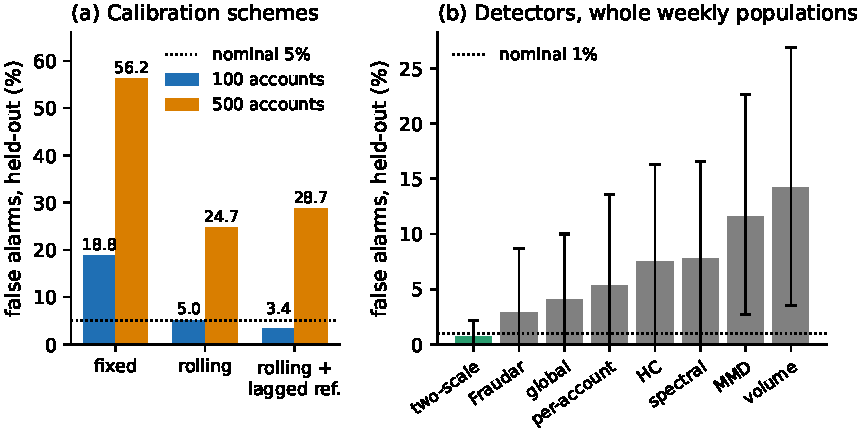
\includegraphics[width=\linewidth]{figs/calibration.pdf}
\caption{Calibration on real traffic. (a) False alarms on held-out weeks for three calibration schemes at a nominal 5\%. Calibrating once on early weeks fails; resampling whole windows from the four preceding weeks, each whitened against its own lagged reference, restores the nominal rate in 100-account windows but not in 500-account windows. (b) Per-detector false alarms at a nominal 1\% over whole weekly populations, with week-clustered intervals: only the two-scale test is calibrated under rolling calibration.}
\label{fig:calib-full}
\end{figure}

A provider's first surprise will be that thresholds do not transfer from one month to the next. Thresholds set on early weeks fired on 12\% of later null weeks against a nominal 1\%: later weeks contain more extreme individual users than any calibration week, and each week's traffic as a whole drifts far from any fixed reference. Resampling \emph{individual accounts} to build a null, the textbook shortcut, also fails, because it destroys the clusters and trends that cross-account tests respond to. What works is resampling \emph{whole historical weeks}, each whitened against its own lagged reference (Figure~\ref{fig:calib-full}a). Even then, over whole weekly populations only the two-scale test stayed calibrated: 0.7\% false alarms at a nominal 1\%, against 2.9\% for Fraudar, 4.1--7.8\% for the global-stream, per-account, Higher Criticism and spectral tests, 11.6\% for MMD and 14.2\% for the volume test (Figure~\ref{fig:calib-full}b). Population sizes vary from week to week, and most statistics move with both size and drift; the two-scale score is a ratio within one group, and both effects largely cancel.

\takeaway{For providers.}{Calibrate on whole historical windows against a lagged reference. A null built by shuffling accounts or queries will look fine in a notebook and fire constantly in production.}

\subsection{What is detectable: coordinated, dataset-like campaigns}
\label{sec:deploy-full}



Table~\ref{tab:deploy} is the core positive result. Campaigns that send prompts from a generated, topically focused dataset were caught most weeks, while no per-account monitor caught anything: volume matching works, and each colluder alone looks ordinary. Broad datasets and real user prompts were not caught---exactly what the barrier predicts for campaigns that look like ordinary users. When the two-scale test fired, the flagged group was almost entirely colluders (precision 1.00 at $K=50$, 0.94--0.96 at $K=10$), but it contained only the 12--31\% of colluders carrying most of the eigenvector's weight. That suits manual review: a handful of accounts that are almost surely colluders, not an enumeration of the campaign.

\paragraph{Its edge is calibration, not ranking.} With all detectors forced to the same realised false-alarm rate by an oracle threshold, the two-scale test caught 0.80 of MetaMathQA campaigns at 1\%, the global stream 0.70 and MMD 0.58; over all operating points, the global stream ranks campaigns slightly \emph{better} (AUC 0.97 against 0.88). The two-scale test's practical advantage is that its threshold transfers across weeks. At stricter oracle false-alarm rates its advantage grows (0.88 at $10^{-3}$ against 0.70 for the global stream and 0.39 for MMD), but the $10^{-3}$ point rests on about three null exceedances and should be read as indicative.

\subsection{What it actually detects: topic shift, not extraction}
\label{sec:mechanism-full}

We designed the two-scale test on the hypothesis that generated distillation sets are concentrated by topic but deduplicated, while benign groups are clumpy. Two ablations, with predictions locked in advance, rejected that story: four rephrasings of each problem cut detection only from 0.88 to 0.80, and exact repeats only from 0.79 to 0.73. What the data support is plainer. Coordinated campaigns of \emph{human-written} GSM8K questions were caught 0.94 of the time---more often than generated MetaMathQA (0.79)---and so were MetaMathQA prompts behind a fixed template (0.94). The test detects \emph{a coordinated group sending prompts concentrated in a topic region that ordinary traffic under-represents}, whatever the reason.

Two consequences matter for a provider. First, simpler source-shift statistics are not enough: a dataset-versus-chat classifier and a topic-concentration statistic applied to the same selected group ranked campaigns moderately (AUC 0.69--0.84) but caught none at a 1\% false-alarm rate; the most dataset-like accounts in every week are benign. Second, the test cannot tell a distiller from a legitimate customer. Benign groups sweeping the GSM8K test set from 3 or 10 accounts triggered it in 79--80\% of weeks, as often as distillation; broad MMLU sweeps did so in only 2--7\%.

\takeaway{For providers.}{Expect evaluation pipelines in the alarms. A firing test is a pointer for review, not a verdict.}

\subsection{Mimicry, and a fix that looks at directions instead of sizes}
\label{sec:mimicry-full}

An attacker who knows a monitor exists has an obvious move: make each colluder look more like a user by mixing natural text into its queries. Mixing half natural prompts into every colluder account, or following every MetaMathQA prompt with a real WildChat follow-up turn, cut two-scale detection from 0.85 to 0.21--0.24 on the development weeks---a fourfold drop, though still well above the false-alarm rate. (On untouched weeks it fell to zero; Section~\ref{sec:holdout}.) We tried four repairs that pool topic cells across accounts---robust per-cell statistics, per-cell lagged scoring with shrinkage, a factor model of cell drift \citep{bai2002determining,ahn2013eigenvalue}, and gating behind the two-scale test. They rank padded campaigns better (AUC up to 0.86) but none reached a usable false-alarm rate at useful power (Appendix~\ref{app:extra}).

The repair that worked came from asking \emph{why} padding works. It dilutes the \emph{size} of each colluder's deviation from normal traffic, but not its \emph{direction}: fifty accounts that each spend half their queries on math still point the same way. The plain matrix $C$ weighs accounts by size, so individually topical benign users dominate it. The centred, hollowed matrix $R_c$ (Section~\ref{sec:monitor}) weighs only directions. With conformal thresholds over all prior weeks, hollowed selection caught MetaMathQA campaigns every week and padded campaigns 0.46--0.48 of the time, against 0.00--0.02 for selection on $C$ under the same calibration, with no false alarm in 960 windows from 24 weeks. Hollowing responds to \emph{many} coordinated accounts: a benign evaluation sweep from ten accounts was flagged 0.97 of the time, one from three accounts 0.42.

Removing the common drift mode also gave a direct reading of the quantity the barrier depends on. Net of each account's own topicality and the week's drift, the top eigenvalue of $R_c$ in real weeks was only 1.14 times that of weeks with queries shuffled across accounts: on these weeks, benign accounts were barely more coordinated than chance. (On the untouched weeks the ratio was 2.22; Section~\ref{sec:holdout}.)

\subsection{Scale: selection fails before the barrier does}
\label{sec:scale-full}

\begin{figure}[t]
\centering
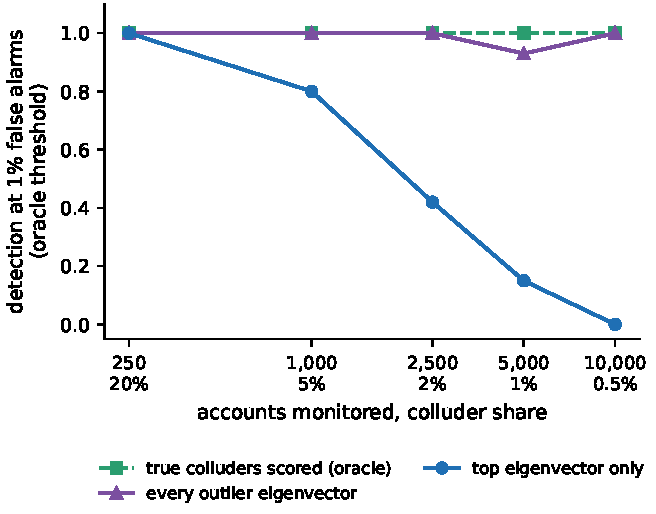
\includegraphics[width=0.62\linewidth]{figs/scale.pdf}
\caption{Scale, with the campaign fixed at 1{,}640 queries over 50 colluders, in populations pooled from account-weeks across the year (oracle thresholds at 1\% false alarms). The detector's own group selection fails as colluders become rarer, although the true colluder set still scores above the threshold at every size; scoring a group from every outlier eigenvector of $R_c$ closes the gap, but only with oracle thresholds.}
\label{fig:scale-full}
\end{figure}

Production populations hold $10^5$ accounts or more, with colluders far below 1\%. Our weekly populations hold a few hundred. We approached the gap in three ways, and the honest summary is negative for deployment.

\paragraph{Smaller colluder shares.} Holding the campaign fixed at 1{,}640 queries and growing the population from 250 to 1{,}000 account-weeks, oracle detection decayed smoothly with colluder share (0.84, 0.60, 0.35 at 20\%, 10\%, 5\%), as the barrier predicts. Calibration was a separate and worse bottleneck: deployed false alarms in these multi-week populations were 14--90\%. Sharding a population into small windows with one colluder each defeated every detector in all 352 shard tests.

\paragraph{Up to $10^4$ accounts.} In populations pooled from account-weeks across the year, the two-scale test's power fell from 1.00 to 0.00 as colluders went from 20\% to 0.5\% (Figure~\ref{fig:scale-full}). But scoring the \emph{true} colluder set with the same statistic exceeded the threshold at every size: the campaign was still there to be seen; the detector simply stopped picking the right accounts. The barrier did not rise as Proposition~\ref{prop:max} would predict; the null threshold of the two-scale score stayed flat between 2.9 and 4.3. Selecting groups from every outlier eigenvector of $R_c$ closed that gap with oracle thresholds: unpadded campaigns were found in 93--100\% of windows up to $10^4$ accounts (0.5\% colluders), padded ones in 77--100\% up to 5{,}000 accounts and 17\% at $10^4$.

\paragraph{Why this is not yet a production result.} Three caveats bind together. These numbers use oracle thresholds; the best deployed calibration of multi-outlier selection reached 5\% false alarms, not 1\%, at 5{,}000--7{,}552 account-weeks, where it caught unpadded campaigns 0.53--1.00 of the time and padded ones 0.03--0.10. Pooling account-weeks across a year removes most same-week benign coordination, so these populations probably understate the barrier. And sparse scans that look for small dense groups did not help: they were captured by individually heavy benign accounts just as the plain spectrum was.

\takeaway{For providers.}{At realistic colluder shares the bottleneck is first \emph{finding} the right accounts and then \emph{calibrating}. We did not solve either at production shares. Query monitoring is far stronger as a complement to metadata linkage: given 30\% of a campaign's colluders, adding the 50 accounts most correlated with them in $R_c$ recovered 96--100\% of all colluders in populations of 2{,}500--10{,}000 accounts (oracle thresholds and known campaign size).}

\subsection{Attacks on the monitor itself}
\label{sec:attacks-full}

\paragraph{Optimising against the statistic.} An attacker that knows the two-scale statistic, and uses its own benign pool to estimate it, ordered MetaMathQA prompts greedily so that their running coarse fingerprint stayed near zero. Without any padding, this cut weekly detection from 0.80 to 0.31.

\paragraph{Choosing who gets flagged.} Giving the 30\% most distinctive queries to five sacrificial accounts kept detection on $C$ at 0.92, but the flagged group then contained none of the other 45 colluders. Banning flagged accounts does not hurt a campaign that chooses whom the detector flags. Hollowed selection resisted this attack on the untouched weeks (Section~\ref{sec:holdout}).

\paragraph{Teaching the monitor that the campaign is normal.} Lagged calibration has a cost the drift results hide. A campaign that ramps up linearly through the eight calibration weeks contaminates both the lagged reference and the calibration windows; at full volume it was caught 0.12 of the time, against 0.95 for the same campaign arriving abruptly. This is the ``boiling frog'' poisoning known from PCA-based traffic anomaly detection \citep{rubinstein2009antidote}. A reference frozen from early weeks recovered some of it (0.44, at 5.2\% false alarms). On the untouched weeks the attack defeated every detector (Section~\ref{sec:holdout}).
